\documentclass[a4paper]{sbgames}               % final
\usepackage[utf8]{inputenc}
%\usepackage[scaled=.92]{helvet}

\usepackage{times}
\usepackage{graphicx}

%% use this for zero \parindent and non-zero \parskip, intelligently.
\usepackage{parskip}

%% the 'caption' package provides a nicer-looking replacement
\usepackage[labelfont=bf,textfont=it]{caption}

\usepackage{url}
\usepackage[]{algorithm2e}
\usepackage{array}
\newcolumntype{L}{>{\centering\arraybackslash}m{3cm}}

%% Paper title.
\title{\textit{Postmortem} do \textit{Flappy Bird}: A Breve Vida de um Fenômeno}


%% Author and Affiliation (multiple authors). Use: and between authors

\author{Fernando L. Souza: Lucas C. Medeiros: Marcos F. Parreiras}

%\affiliation{Departamento de Computa\c{c}\~{a}o \\
%        Centro Federal de Educa\c{c}\~{a}o Tecnol\'{o}gica de Minas Gerais \\
%        Belo Horizonte, Brasil
%}

\affiliation{ Centro Federal de Educa\c{c}\~{a}o Tecnol\'{o}gica de Minas Gerais, Departamento de Computa\c{c}\~{a}o, Brasil
}

\contactinfo{nandolcs@hotmail.com \\
             *cmedeiros.lucas@gmail.com \\
             *marcosfparreiras@gmail.com
}
%\contactinfo{author1@email.com \\
%             author2@email.com
%}
%% Keywords that describe your work.
\keywords{postmortem. flappy bird. aplicativos móveis. jogos digitais.}

%% Start of the paper
% Attention: As you need to insert EPS images in Postscript, 
% you need to insert PDF images into PDFs. 
% In the text, extensions cancbe omitted (latex use .eps, pdflatex get .pdf) 
% To convert them: epstopdf myimage.eps
\begin{document}

%\teaser{
 % 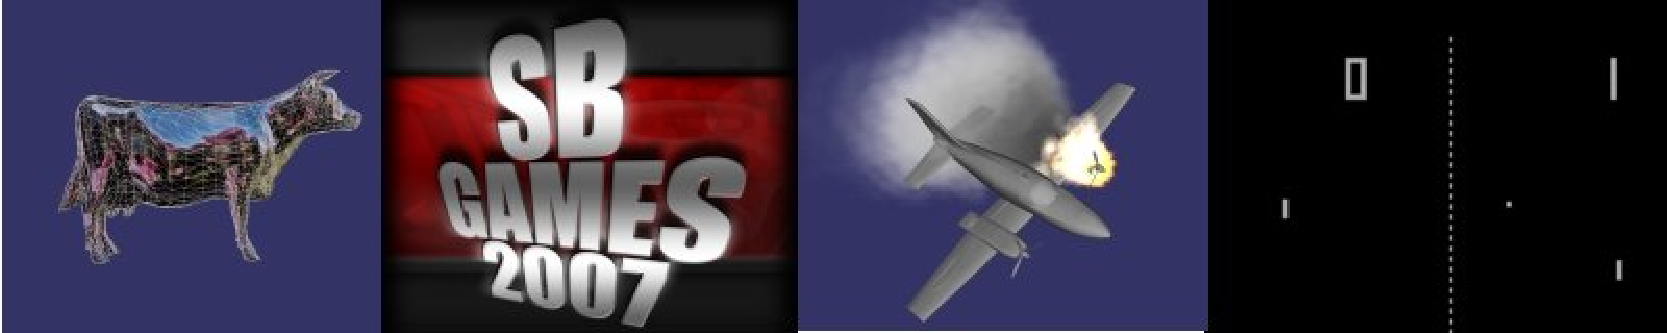
\includegraphics[width=\linewidth]{sample.pdf}
  %\caption{Optional image}
%}

%% The ``\maketitle'' command must be the first command after the
%% ``\begin{document}'' command. It prepares and prints the title block.

\maketitle

%% Abstract section.

%\begin{abstract}
%\end{abstract}
\section*{Resumo}
O jogo \textit{Flappy Bird} foi um fenômeno mundial no contexto de jogos para plataforma \textit{mobile}. Em meio a um mercado tão competitivo, este artigo trata dos aspectos que levaram este simples jogo ao posto de mais jogado em vários lugares do mundo e com arrecadaçao superior a cinquenta mil dólares por mês sem nenhum tipo de campanha publicitária além de relacionar como as decorrências disso foram determinantes para que o jogo tivesse um final tão repentino quanto sua ascensão.

%% The ``\keywordlist'' command prints out the keywords.
\keywordlist
\contactlist

\section{Introdução}
\label{sec:introducao}

Introdução

Com a chegada da plataforma mobile, a possibilidade de se alcançar grande sucesso com software aumentou significativamente. No caso dos aplicativos desenvolvidos para esta plataforma, o software está sempre ao alcance do usuário final, permitindo que seja utilizado a partir de um simples toque.

O mercado de jogos é um dos que tem se aproveitado desta versatilidade e, com isso, vários são os casos de jogos que vêm ganhando grande popularidade e alcançando a casa dos milhões de downloads, como é o cado, por exemplo, dos jogos \textit{Candy Crush Saga} e \textit{Clash of Clans}. Um caso bastante especial de jogo a se destacar em meio a este mercado tão concorrido foi o \textit{Flappy Bird}: um dos jogos mais emblemáticos e icônicos desde o início deste novo mercado mobile. Possuindo uma estrutura extremamente simples, este jogo teve uma ascensão meteórica, alcançando o topo das principais lojas de aplicativos, \textit{Google Play} e \textit{App Store}, e chegando a arrecadar cerca de cinquenta mil dólares por dia a partir de anúncios no aplicativo \cite{Warren2014}. Após tamanho sucesso, seu fim foi tão repentino quanto seu surgimento, como é relatado na próxima seção.






\section{Uma Breve História do Jogo}
\label{sec:historia}

A origem do jogo \textit{Flappy Bird} data de novembro de 2012, quando o vietnamita Dong Nguyen divulgou em seu \textit{Twitter} uma primeira imagem divulgando o início da criação de mais um jogo \cite{Warren2014}. Nguyen era o único funcionário do estúdio de jogos .Gear, fundado por ele pŕopio \cite{Harvard2014}. Após a fase de refinamento, o jogo, originalmente nomeado \textit{Flappy Flappy} foi renomeado para \textit{Flappy Bird} e lançado na \textit{App Store} em abril de 2013. A alteração no nome se deveu ao fato de, na época, já existir um jogo na loja com o nome \textit{Flappy Flappy}.

O jogo se manteve no anonimato até outubro de 2014, quando ainda ocupava a posição número 1469 dentre os aplicativos da categoria Família na \textit{App Store}. Nos mês de novembro, o jogo começou a se popularizar a partir de divulgação de usuários no \textit{Twitter} e no \textit{Facebook}, fazendo com que, no início de dezembro, já ocupasse a posição 74 na categoria Família, e sendo o aplicativo número 1308 nos Estados Unidos \cite{Warren2014}.

Devido ao seu extremo nível de dificuldade, usuários de redes sociais passaram a postar publicamente seus casos de amor e ódio com o jogo, elevando sua visibilidade ainda mais e fazendo com que no dia dez de janeiro de 2014, alcançasse o \textit{top 10} da \textit{App Store} nos EUA. Neste mesmo mês, no dia vinte e dois, foi lançada na \textit{Google Play} a versão do jogo para \textit{Android} e em menos de uma semana ele alcançou o posto de aplicativo mais baixado da loja \cite{Warren2014}.

Os mais de cinquenta milhões de downloads do jogo fizeram com que a mídia focasse bastante em seu criador, Dong Nguyen, que chegou inclusive a ser acusado de usar técnicas ilegais para aumentar o número de \textit{reviews} do seu jogo. Segundo as acusações, ele estaria utilizando um robô para gerar \textit{reviews} automaticamente para, desta forma, promover seu jogo mais rapidamente.Estas acusações entretanto nunca foram confirmadas \cite{Warren2014}.

Outra prova do sucesso do jogo foi o fato de alcançar o primeiro lugar na \textit{App Store} em 53 países diferentes, mostrando que seu sucesso foi a nível global \cite{Warren2014}.

Neste momento, o jogo estava gerando cerca de U\$\$ 50.000,00 por dia com anúncios e Nguyen já começara a sucumbir a toda a pressão sobre ele e sobre seu jogo. Com isto, no dia oito de fevereiro de 2014, ele postou uma mensagem oficial no seu \textit{Twitter} informando aos usuários do jogo que ele seria tirado do ar no dia seguinte. Muitos acreditram que seria uma questão de \textit{marketing} ou que ele tivera algum problema legal relacionado ao jogo. Ambas as suposições estavam erradas: Nguyen tirou o jogo da loja porque, segundo ele, as pessoas estavam deixando de viver suas vidas para jogar o jogo que ele tinha criado \cite{Warren2014}.

Desta forma, no dia nove de fevereiro, vinte e oito dias após entrar no \textit{top 10}, o jogo foi de fato retirado do ar, acumulando mais de cinquenta milhões de \textit{downloads} e mais de dezesseis milhões de \textit{tweets} relacionados \cite{Warren2014}.

\section{Componentes}
\label{sec:componentes}

%Antes de se fazer uma an�lise do que levou o jogo \textit{Flappy Bird} a ter tanto sucesso, primeiro devem se introduzir seus componentes.
%Antes de se fazer uma an�lise do que levou o jogo \textit{Flappy Bird} a ter tanto sucesso, primeiro devem-se introduzir seus componentes.

\subsection{Arte}
A arte do jogo � extremamente simples, sendo desenvolvida em oito \textit{bits} e com pequenas varia��es rand�micas a cada turno: a cor do p�ssaro e o c�u tamb�m, dando ideia de dia ou noite. Apesar de os efeitos serem simples, s�o tamb�m agrad�veis. Os obst�culos do jogo representados por canos, bem como outros elementos do cen�rio, seguem o padr�o dos jogos da franquia do \textit{Super Mario}. Outro ponto de simplicidade na arte do jogo � o fato de a paisagem de fundo ser totalmente est�tica, o que se tornou extremamente raro num contexto em que o efeito de rolamento \textit{parallax} se tornou t�o difundido \cite{Eldic2014}.

\subsection{Sons}
Os sons do jogo se limitam �queles que representam seus evento: impulsionar o p�ssaro, passar por um obstaculo e morrer. Com isso, o jogo n�o apresenta nenhuma m�sica de fundo, se mostrando bastante simples tamb�m neste aspecto \cite{Eldic2014}.

\subsection{\textit{Game Design}}
Os mecanismos do \textit{Flappy Bird} s�o extremamente simples, provados e fortes, sendo ele um jogo de helic�ptero em que, a partir de um toque, o objeto controlado sobe e, quando n�o se toma nenhuma a��o, ele cai devido � a��o da gravidade \cite{Eldic2014}.

O \textit{Fappy Bird}, entretanto, incorpora algumas caracter�sticas que tornam este jogo ainda mais interessante: a primeira delas � o fato de n�o se poder segurar o dedo apertado, fazendo com que seja sempre necess�rio apertar a tela novamente para evitar que o p�ssaro caia. Isso aumenta o n�vel de dificuldade do jogo, o tornando mais desafiador. Uma segunda caracter�stica � o fato de o jogo n�o ter sua dificuldade alterada em nenhum momento, com velocidade e tamanho dos obst�culos sempre constantes \cite{Eldic2014}.

\subsection{\textit{Marketing}}
Nenhuma campanha de \textit{marketing} foi feita partindo de Nguyen. Sua divulga��o foi totalmente baseada no sucesso em que se tornou, a partir de cada vez mais men��es nas redes sociais como \extit{Facebook} e \textit{Twitter} \cite{Eldic2014}.

\subsection{Monetiza��o}
A monetiz���o do \textit{Flappy Bird} foi baseada nos an�ncios exibidos durante o jogo. Com isso, a distribui��o do jogo foi gratuira, durante todo o tempo em que esteve dispon�vel. O sucesso do jogo fez com que as arrecada��es com an�ncios ultrapassassem os cinqenta mil d�lares por dia \cite{Eldic2014}.



Antes de se fazer uma análise do que levou o jogo \textit{Flappy Bird} a ter tanto sucesso, primeiro devem-se introduzir seus componentes, que tiveram influência determinante nele.

\subsection{Arte}
A arte do jogo é extremamente simples, sendo desenvolvida em oito \textit{bits} e com pequenas variações randômicas a cada turno: a cor do pássaro e o céu também, dando ideia de dia ou noite. Apesar de os efeitos serem simples, são também agradáveis. Os obstáculos do jogo representados por canos, bem como outros elementos do cenário, seguem o padrão dos jogos da franquia do \textit{Super Mario}. Outro ponto de simplicidade na arte do jogo é o fato de a paisagem de fundo ser totalmente estática, o que se tornou extremamente raro num contexto em que o efeito de rolamento \textit{parallax} se tornou tão difundido \cite{Eldic2014}.

\subsection{Sons}
Os sons do jogo se limitam àqueles que representam seus evento: impulsionar o pássaro, passar por um obstaculo e morrer. Com isso, o jogo não apresenta nenhuma música de fundo, se mostrando bastante simples também neste aspecto \cite{Eldic2014}.

\subsection{\textit{Game Design}}
Os mecanismos do \textit{Flappy Bird} são extremamente simples, provados e fortes, sendo ele um jogo de helicóptero em que, a partir de um toque, o objeto controlado sobe e, quando não se toma nenhuma ação, ele cai devido à ação da gravidade \cite{Eldic2014}.

O \textit{Fappy Bird}, entretanto, incorpora algumas características que tornam este jogo ainda mais interessante: a primeira delas é o fato de não se poder segurar o dedo apertado, fazendo com que seja sempre necessário apertar a tela novamente para evitar que o pássaro caia. Isso aumenta o nível de dificuldade do jogo, o tornando mais desafiador. Uma segunda característica é o fato de o jogo não ter sua dificuldade alterada em nenhum momento, com velocidade e tamanho dos obstáculos sempre constantes \cite{Eldic2014}.

\subsection{\textit{Marketing}}
Nenhuma campanha de \textit{marketing} foi feita partindo de Nguyen. Sua divulgação foi totalmente baseada no sucesso em que se tornou, a partir de cada vez mais menções nas redes sociais como \textit{Facebook} e \textit{Twitter} \cite{Eldic2014}.

\subsection{Monetização}
A monetizãção do \textit{Flappy Bird} foi baseada nos anúncios exibidos durante o jogo. Com isso, a distribuição do jogo foi gratuira, durante todo o tempo em que esteve disponível. O sucesso do jogo fez com que as arrecadações com anúncios ultrapassassem os cinqenta mil dólares por dia \cite{Eldic2014}.

\section{Fórmula do Sucesso}
\label{sec:sucesso}

Apesar da grande simplicidade do jogo, ele alcançou um sucesso estrondoso. Os principais motivos disso são:

\begin{itemize}
\item[É simples, mas muito difícil]: Todo o funcionamento do jogo é baseado num único controle: o clique na tela. Com isso, não é necessária nem mesmo uma tela de instruções permitindo que qualquer pessoa que tenha o jogo em mãos, possa jogá-lo. O contraponto à simplicidade do jogo surge no seu nível de dificuldade extremamente elevado, fazendo com que o jogo seja fácil de se aprender, mas difícil de se dominar. A simplicidade faz com que os jogadores se cobrem na obtenção de melhores resultados, que são difíceis de se conquistar. Isso dá ao jogo o tom desafiador e viciante \cite{Dino2014}.

\item[Se baseia na nostalgia]: A aparência do jogo remete muito à franquia \textit{Super Mario}, fazendo com que uma simpatia quase instantânea seja compreendida pelos fãs da famosa franquia quando jogam o \textit{Flappy Bird} \cite{Dino2014}.

\item[Não possui atalhos]: Ao contrário de diversos jogos atuais que oferecem facilidades a partir de compras dentro dos aplicativos, como dobrar pontuação e reduzir dificuldade por exemplo, o \textit{Flappy Bird} não oferece nenhuma circunstância desigual. Com isso, a pontução obitda pelo jogador é exatamente a merecida por ele, acirrando disputas entre amigos e tornando o jogo um fenômeno social \cite{Dino2014}.

\end{itemize}







\section{Conclusão}
\label{sec:conclusao}

O \textit{Flappy Bird} foi um fenômeno mundial no contexto de jogos para a plataforma \textit{mobile}. Tendo sido desenvolvido por uma única pessoa, alcançou o posto de aplicativo mais baixado nas principais lojas de aplicativos móveis do mundo apesar de sua grande simplicidade, superando largamente o sucesso de jogos desenvolvidos por grandes corporações.

Seu sucesso foi devido a um conjunto de fatores dentre os quais se compensa destacar a própria simplicidade do jogo. A jogabilidade a partir de um único comando, aliado ao seu grande nível de dificuldade fez com que milhões de pessoas se sentissem frustradas consigo mesmas, incentivando assim seu uso constante na tentativa de melhorar as marcas pessoais, além de contribuir para as inúmeras divulgações que foram feitas ao redor de todo o mundo quando algum jogador alcançava um placar alto, fazendo do jogo um fenônemo social.

Mesmo sem nenhuma campanha de \textit{marketing}, o jogo alcançou arrecadação de mais de cinquenta mil dólares por dia sobre os anúncios que nele eram mostrados, o que somente foi possível devido ao fato de o número de jogadores chegar à marca incrível de cinquenta milhões de usuários.

Um dos pontos que o fez se tornar um fenômeno, foi seu pico de existência, tendo tido uma ascensão meteórica, e tendo sido removido do ar menos dia trinta dias após alcançar o \textit{top 10} da \textit{App Store}, devido às repercursões que a fama do jogo teve na vida do seu criador.

Com isso, pode-se ver quantos aspectos foram relacionados ao seu sucesso mas também as repercursões que ele trouxe.




\bibliographystyle{sbgames}
\bibliography{template}
\end{document}
